%Questo è il preambolo, dove si inseriscono i pacchetti e le impostazioni che servono per compilare il documento. Quanto scritto dopo il simbolo '%' è solo un commento e serve a fini dimostrativi.

\documentclass[11pt]{article}
\linespread{1.6} %interlinea
\pagestyle{plain}
\usepackage{geometry} %margini
\geometry{a4paper, top=3cm, bottom=3cm, left=3cm, right=3cm, bindingoffset=5mm}
\usepackage{graphicx}
\graphicspath{immagini/}
\usepackage{multicol} %più colonne
\usepackage{ragged2e} %allineamento testo

\usepackage[italian]{babel} %lingua principale

\usepackage{minitoc} %mini sommario a inizio capitolo
\nomtcrule 
\addto{\captionsitalian}{% Making babel aware of special titles
  \renewcommand{\mtctitle}{Sommario}
}




\usepackage[sorting=none,backend=biber]{biblatex} %bibliografia
\defbibheading{bibbysubsect}{\section*{}}
\addbibresource{bibliografia.bib}





\usepackage[demo]{graphicx}
\usepackage{subcaption}
\usepackage{comment}



\begin{comment}


\renewcommand{\familydefault}{\sfdefault}



\end{comment}



    


    


    








\usepackage{xpatch}
\usepackage{blindtext}
\usepackage{url}


\makeatletter

\xpatchcmd{\@makeschapterhead}{%
  \Huge \bfseries  #1\par\nobreak%
}{%
  \Huge \bfseries\centering #1\par\nobreak%
}{\typeout{Patched makeschapterhead}}{\typeout{patching of @makeschapterhead failed}}


\xpatchcmd{\@makechapterhead}{%
  \huge\bfseries \@chapapp\space \thechapter
}{%
  \huge\bfseries\centering \@chapapp\space \thechapter
}{\typeout{Patched @makechapterhead}}{\typeout{Patching of @makechapterhead failed}}

\makeatother

\usepackage{fancyhdr}
\usepackage[export]{adjustbox}



\usepackage{hyperref} %hyperlink
\hypersetup{
    colorlinks=true,
    citecolor=cyan,
    linkcolor=black,
    urlcolor=black,
    pdftitle=EYE TRACKER,
    pdfauthor= Filippo Veronesi,
    }

\usepackage{booktabs} %per le tabelle
\usepackage{multirow}
\usepackage[table,xcdraw]{xcolor}
\usepackage{graphicx}

\usepackage{lscape}
\usepackage{float}
\usepackage{wrapfig}
\usepackage{epigraph}
\usepackage{fancyhdr}
%Da qui in poi inizia il documento.
\begin{document}
\begin{titlepage} %Cambia i valori in \vspace{} per ottenere un risultato perfetto

\begin{center}
	{\upshape\Large\bfseries ALMA MATER STUDIORUM - UNIVERSITÀ \\ DI BOLOGNA \par}

	\vspace{0,8cm}
		\hrule
	\vspace{0,9cm}
	\vspace{0,3cm}
	{\upshape\small DIPARTIMENTO DI INFORMATICA - SCIENZA E INGEGNERIA\par} 
	\vspace{0,2cm}
	\vspace{0.5cm}
	
	\vspace{1,4cm}
	{\upshape\large\bfseries PROGETTO E ATTIVITÀ PROGETTUALE IN SISTEMI DIGITALI M\par}
	
			
	\vspace{2.3cm}

	{\upshape\large\bfseries EYE TRACKER\par}
	\vspace{2.5cm}
	{\upshape\large\bfseries Luigi di Nuzzo - Daniele Foschi - Filippo Veronesi\par}
	\end{center}
	
	
	
	\vfill
	\hrule
% Bottom of the page
	{\begin{center}
	\vspace{0.3cm}
	     \schape\large Anno Accademico 2021/2022 \\
	     \schape\large Maggio 2022
	\end{center}}

\end{titlepage}


\fancyhf{}
\pagestyle{fancy}
\newcommand{\headeright}{PROGETTO E ATTIVITÀ PROGETTUALE SISTEMI DIGITALI M}
\renewcommand{\headrulewidth}{0.4pt}
\fancyheadoffset{0pt}
\fancyhead[R]{Overleaf}
\renewcommand{\footrulewidth}{0.4pt}

\fancyfoot[R]{Luigi di Nuzzo - Daniele Foschi - Filippo Veronesi}
\rhead{\scshape \footnotesize \headeright}
\chead{\shorttitle}






\clearpage
\null
\thispagestyle{empty}
\clearpage

\newpage







\cleardoublepage



\newpage

\tableofcontents


\newpage


\listoffigures



\newpage


\newpage
\fancyfoot[L]{\thepage}
\setcounter{page}{1}
\section{Introduzione}
Questo progetto prevede la realizzazione di un applicativo Android che, sfruttando una rete neurale, sia in grado di riconoscere il volto dell’utente e di questo ultimo, anche i propri occhi. Il sistema sfrutterà un modello di rete neurale
addestrato in modo tale da essere in grado di riconoscere i visi e gli occhi di uno o più utenti grazie ad un dataset di 10 mila immagini di visi umani.
L’applicativo permetterà di svolgere un filtraggio "live", cioè aprendo la camera frontale ed esterna dello smartphone e individuando real-time gli occhi dell’utente.
\newline
Inoltre, è stato implementato un gioco composto da un Quiz di 4 domande aiutato da un tool di calibrazione. L'utente tramite il riconoscitore di occhi è in grado di rispondere ad una certa domanda spostando, tramite gli occhi e il cellulare, un puntatore verso la risposta giusta posta ai 4 angoli del dispositivo. In caso di risposta corretta, viene posta un'ulteriore domanda, altrimenti si viene avvertiti della domanda sbagliata tramite un alert.
\newline \newline
Tale caso di studio è un classico esempio di applicazione di Machine Learning e il software farà ricorso a una rete neurale convoluzionale (CNN). Tale scelta è dovuta al fatto che una rete neurale rappresenta il modo più comodo e pratico per problemi di object detection, come quello di questa attività in cui vengono individuati gli occhi.
\newline \newline
L’applicativo, inoltre, è pensato per la piattaforma Android e quindi tale progetto pone attenzione anche all’uso di risorse in quanto dovrà funzionare su smartphone, ovvero dispositivi embedded.

\newpage

\section{Rete Neurale}
L’obiettivo primario di questo task è produrre un modello di rete neurale addestrata in grado di riconoscere gli occhi di una o più persone. A tal scopo si è utilizzato un modello messo a disposizione dalla libreria \textit{TensorFlow 2 Detection Model Zoo} ottimizzato per il training di modelli specifici per object detection di immagini. Visto l’ambito dei sistemi embedded nel quale il progetto complessivo si colloca si è optato per un modello SSD MobileNet\footnote{SSD MobileNet V2 FPNLite 640x640}, una CNN pensata per dispositivi mobile. MobileNet è il primo modello di computer vision pensato per dispositivi embedded basato su TensorFlow. MobileNet è sufficientemente leggera e veloce da essere eseguita su smartphone senza consumo di risorse eccessivo mantenendo comunque una precisione adeguata.


\subsection{Dataset}
Per il training del modello si è utilizzato un dataset pubblico rilasciato da Google (LINK DA INSERIRE) contenente 10 mila immagini di visi umani, dove ogni foto conteneva da uno a più visi umani.
\newline
Oltre alle immagini il dataset conteneva un utile file Excel che indicava le coordinate della posizione degli occhi delle persone all'interno dell'immagine.
\newline \newline
Prima dell'addestramento della rete era però necessario convertire questi dati di input in file XML in modo tale da poterli poi convertire in TFRecord, utili per TensorFlow. Per questo motivo è stato implementato uno script Java in grado di creare un file XML per ogni foto del dataset con al suo interno le informazioni geografiche della posizione degli occhi. 
Inoltre, si è reso necessario compilare il file labelmap.pbtxt con al suo interno i nomi e gli id di nostri oggetti da riconoscere: nel nostro caso un solo item di id pari a 1 e con nome "Human eye".
\begin{figure}[h]
\caption{labelmap.pbtxt}
\centering
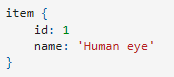
\includegraphics[scale=1]{img/item.png}
\end{figure}


\subsection{Training}
Si è quindi proceduto all’addestramento della rete tramite Python usando TensorFlow e le API di Keras. Si è reso necessario modificare il file \textit{pipeline.config} adattandolo alle nostre esigenze: 
\begin{itemize}
    \item \textit{numclasses} che corrisponde al numero di item da identificare;
    \item \textit{path} vari da adattare al nostro workspace, tra cui il path per i checkpoint, per i record di input e per il labelmap.
\end{itemize}
\newline
Durante il procedimento di training si sono tenuti controllati i valori della nostra rete. In particolare, abbiamo usato \textbf{Tensorboard}: un framework grafico utile a capire l'andamento della nostra rete, infatti abbiamo avuto modo di controllare ad ogni training le performance della nostra rete di machine learning.
\newline
TensorBoard fornisce la visualizzazione e gli strumenti necessari per la sperimentazione del machine learning:
\begin{itemize}
    \item Monitoraggio e visualizzazione di metriche come perdita e precisione;
    \item Visualizzazione del grafico del modello (operazioni e livelli);
    \item Visualizzazione degli istogrammi di pesi, distorsioni o altri tensori man mano che cambiano nel tempo.
\end{itemize}



INSERIRE IMMAGINI GRAFICI
\newline
Si è ottenuto in output un modello addestrato e pronto all’uso.
\newline \newline
Prima di testare direttamente su Android, abbiamo deciso prima di testare e analizzare la nostra nuova rete utilizzando la libreria Matplotlib, utile per visualizzare graficamente via shell i nostri risultati. In particolare abbiamo usato \textbf{Tkinter}, l'unico framework GUI incluso nella libreria standard di Python.
\newline
A fini di testing si è preso ad esempio il volto di un
personaggio pubblico, quello di Albert Einstein, e anche un'immagine contenente più persone in modo tale da poter verificare la correttezza e la precisione della rete anche in condizioni più difficili. 



\begin{figure}
\begin{subfigure}{0.5\textwidth}
  \centering
  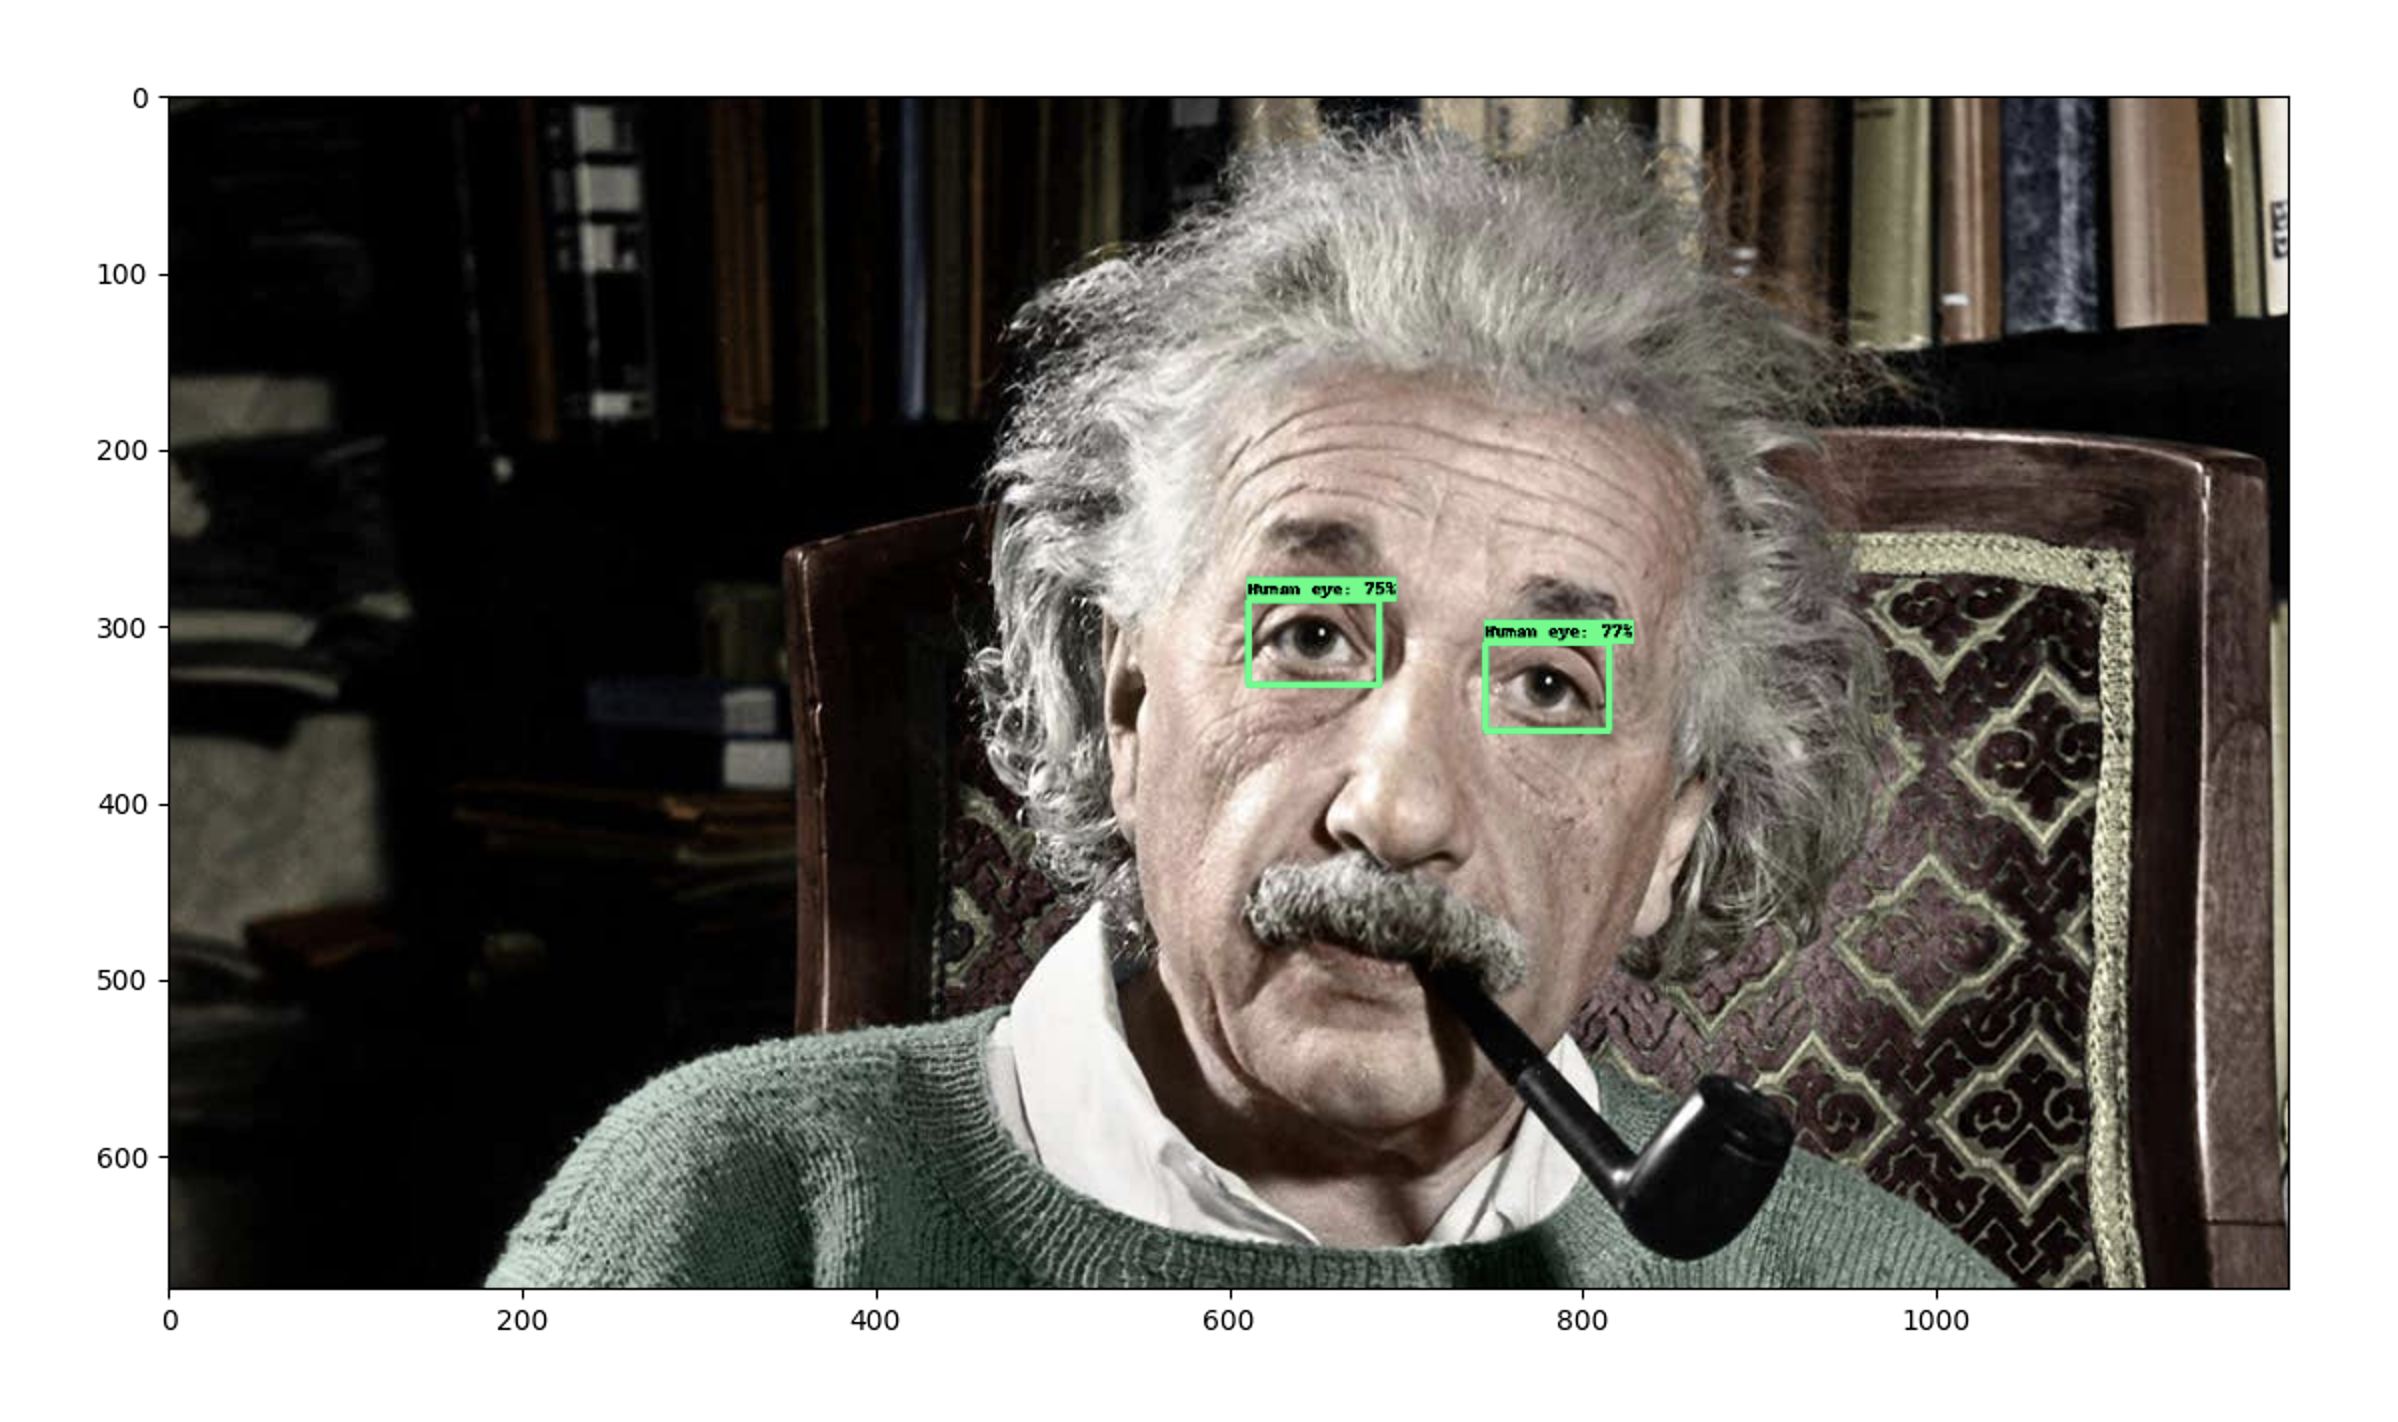
\includegraphics[width=1\linewidth]{img/einstein.png}
  \caption{Test personaggio famoso}
  \label{fig:sfig1}
\end{subfigure}%
\begin{subfigure}{0.5\textwidth}
  \centering
  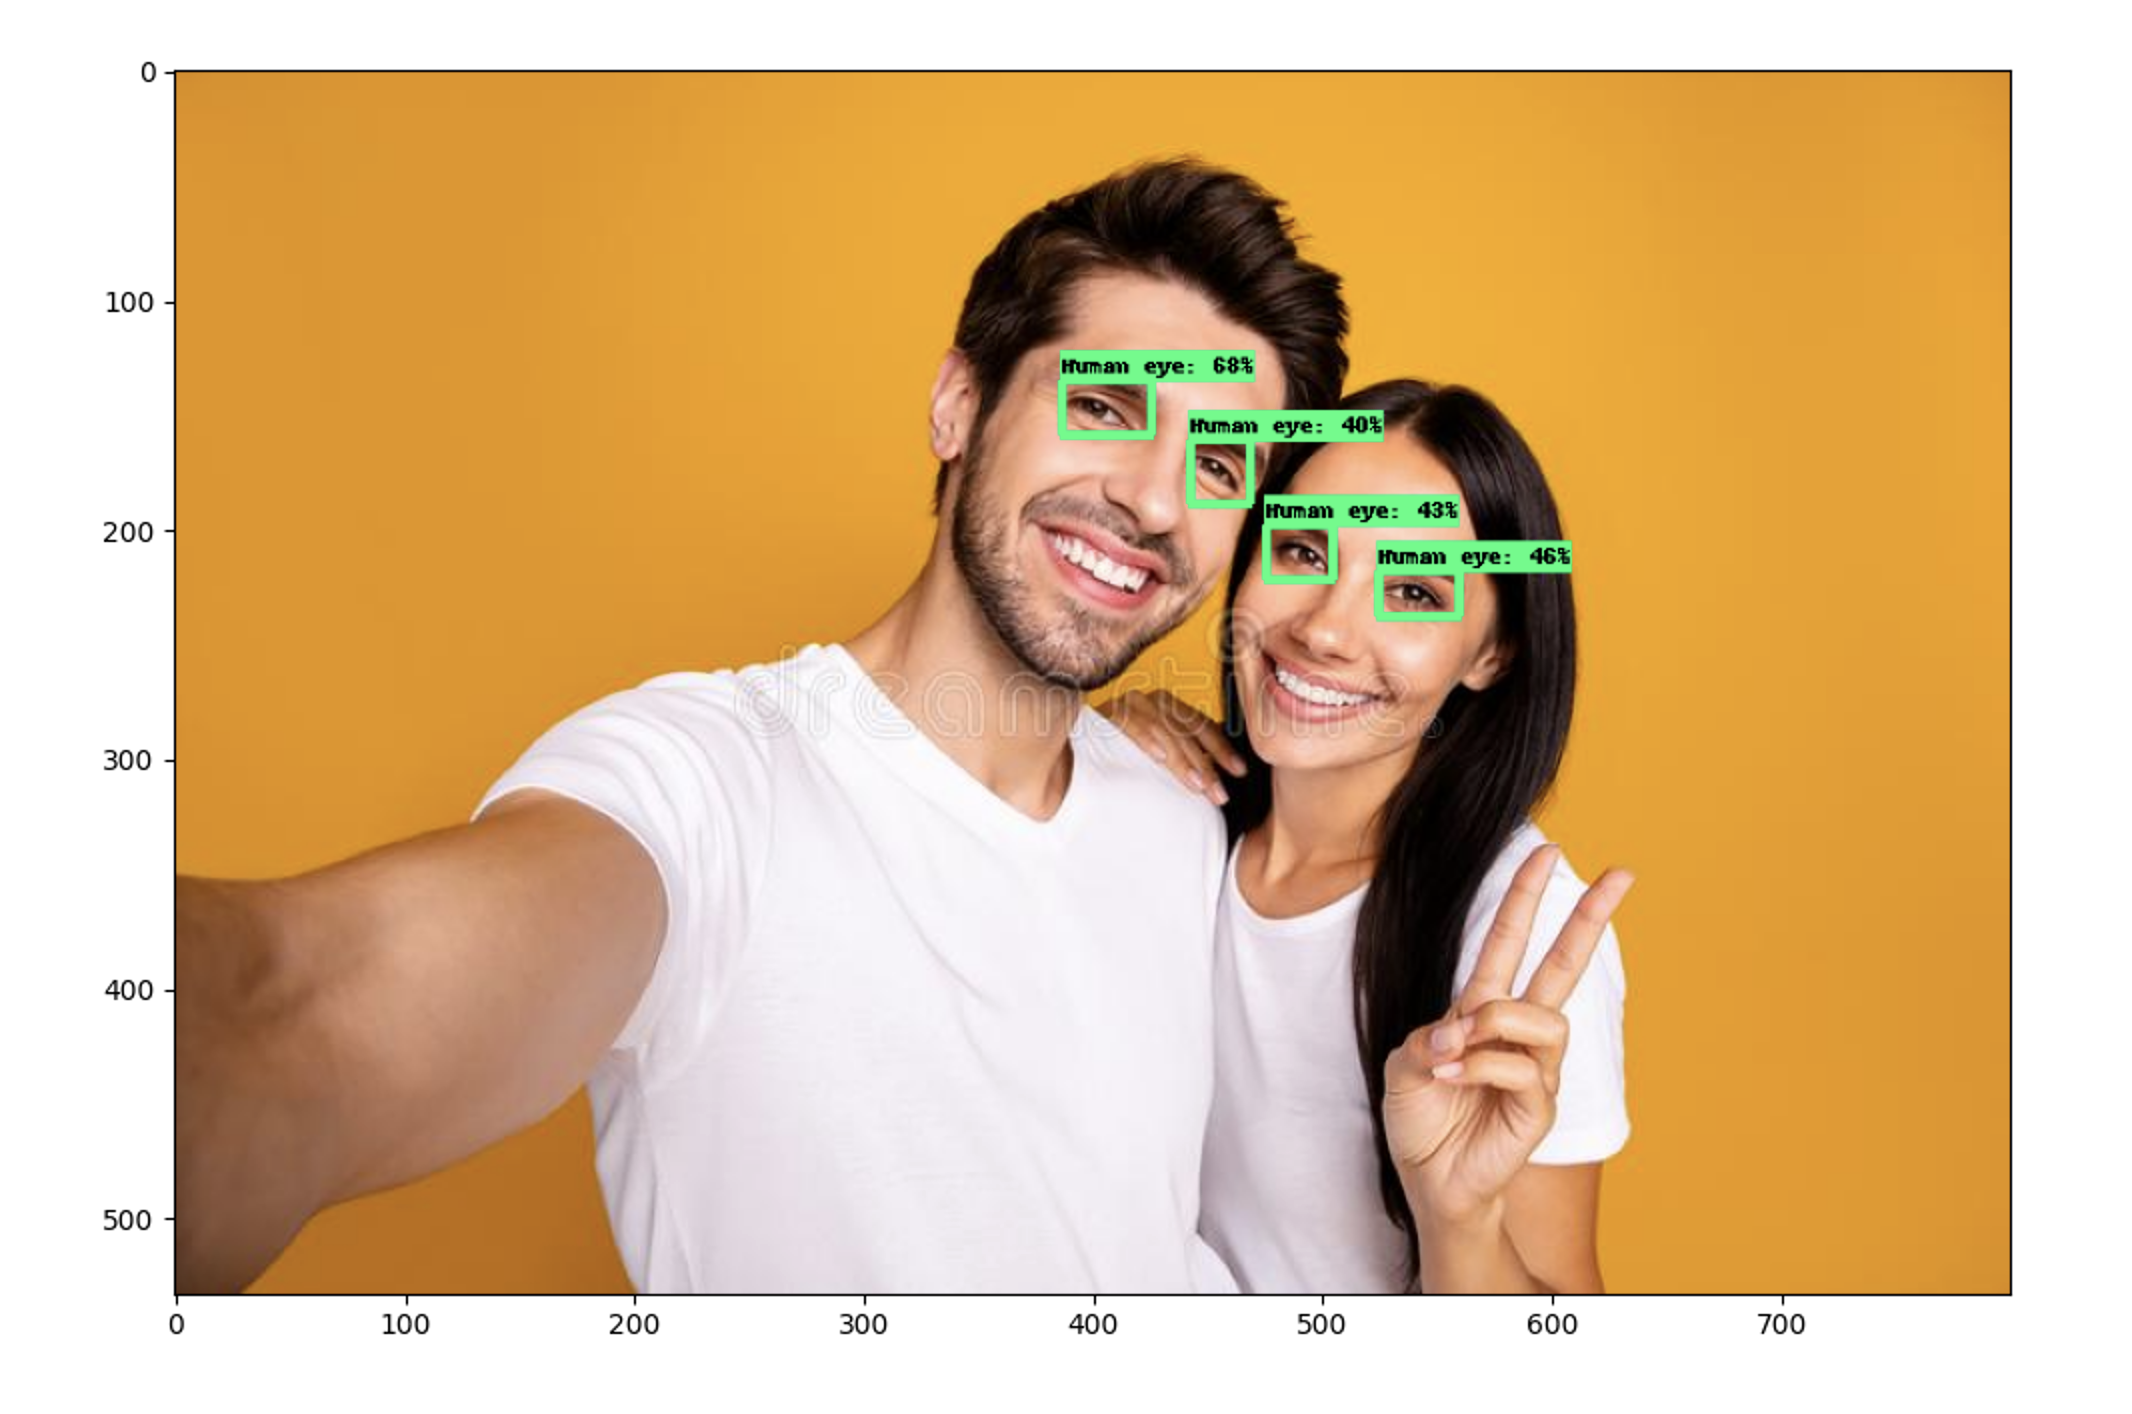
\includegraphics[width=1\linewidth]{img/gruppo.png}
  \caption{Test multiplo}
  \label{fig:sfig2}
\end{subfigure}
\caption{Testing GUI TkAgg}
\label{fig:fig}
\end{figure}

\newpage
\subsection{TFLite}
Dopo esserci accertati che la rete funzionasse correttamente e avesse dei livelli di precisione sopra una certa soglia, si è ottenuto in output un modello addestrato
e pronto all’uso, che poi è stato convertito e quantizzato in un formato adatto ai sistemi embedded, quello di TensorFlow Lite.
\subsubsection{Metadata}
Per un corretto funzionamento della rete neurale all'interno di Android, tflite richiede che venga generato anche un file Metadata che contiene le informazioni necessarie per pre-processare le immagini. Questo file si rende necessario in quanto i nostri tensori di input sono di tipo kTfLiteFloat32. 
\newline
Una volta generato questo nuovo file metadata.tflite siamo pronti ad importarlo all'interno della nostra applicazione Android come file di Machine Learning "ml".


\newpage
\section{Progetto Android}
L'applicazione Android una volta avviata presenta la seguente interfaccia:

\begin{figure}[h]
\caption{Homepage App }
\centering
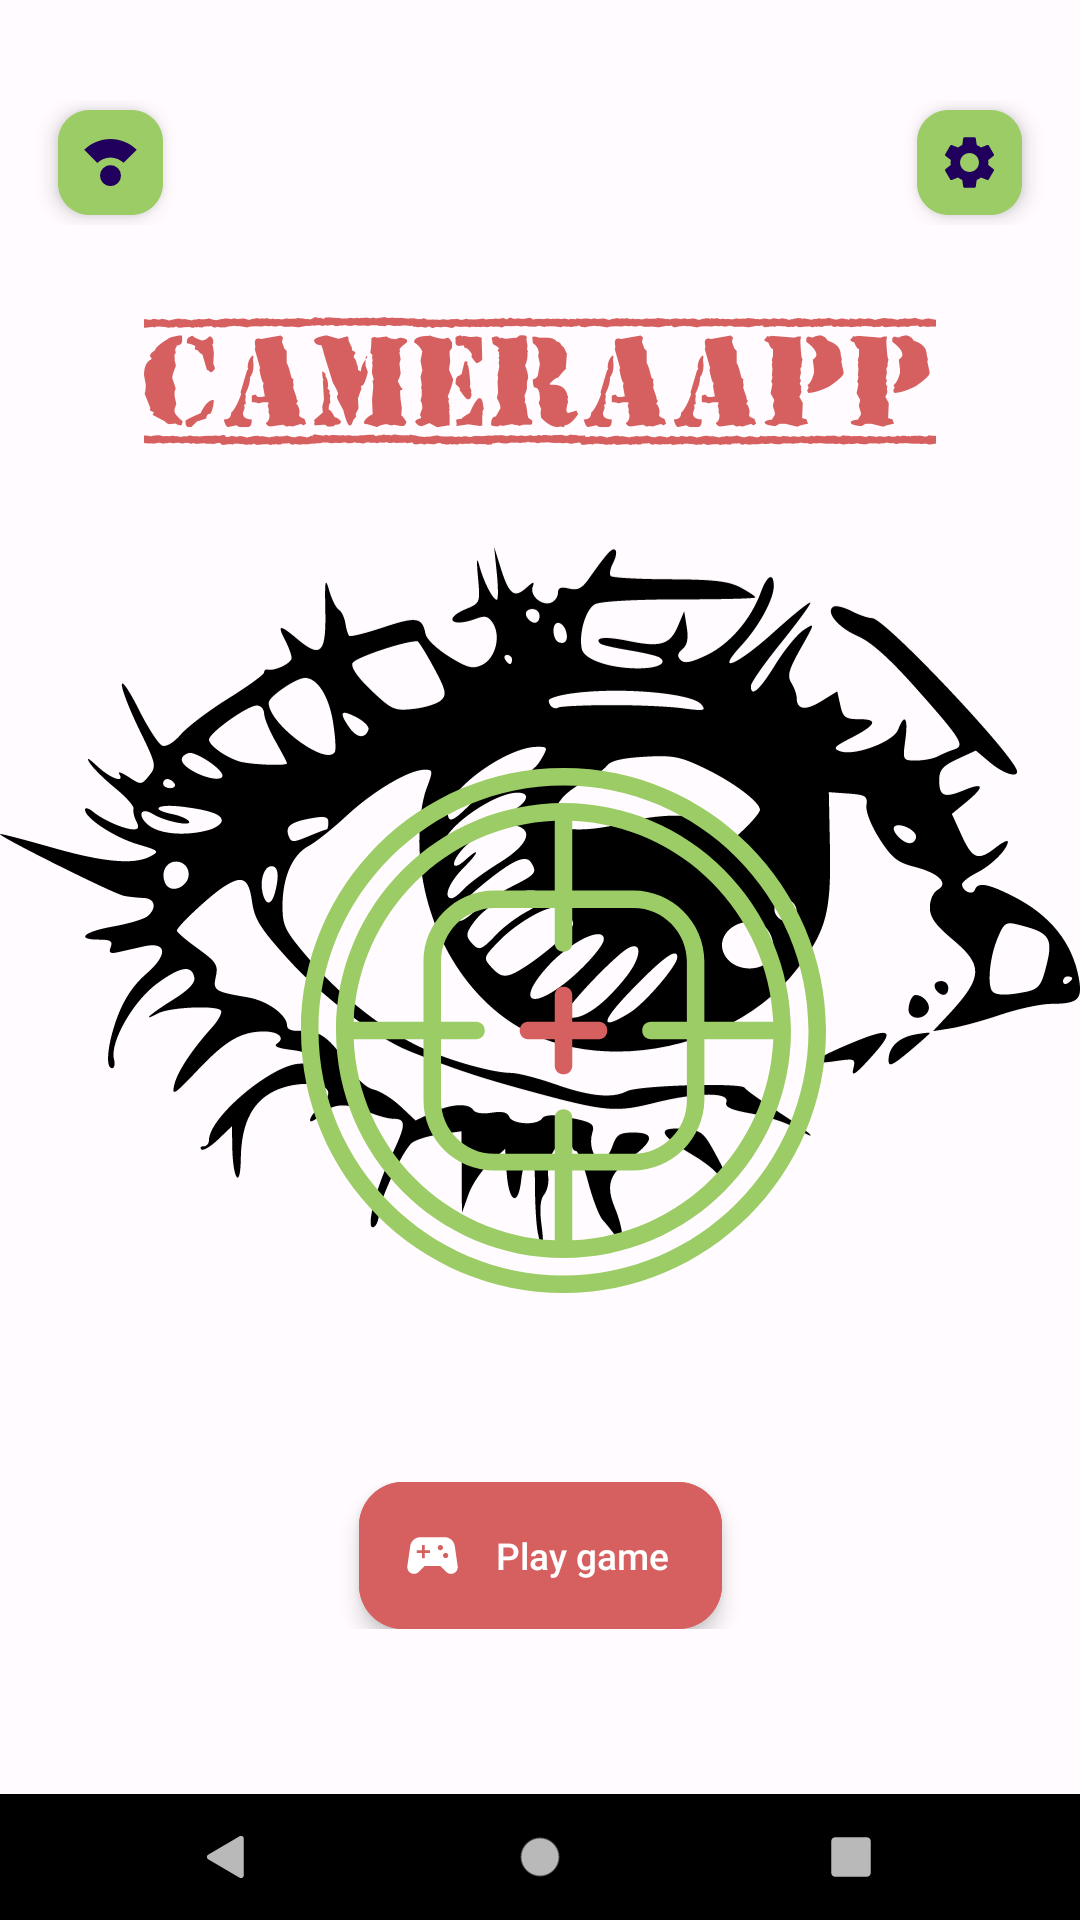
\includegraphics[scale=0.18]{img/home.png}
\end{figure}

Sono da segnalare i 3 principali bottoni dell'applicazione:
\begin{itemize}
\item \textbf{Nerd Mode} in alto a destra;
\item \textbf{Calibration} in alto a sinistra;
\item \textbf{Play Game} al centro dello schermo.
\end{itemize}

\subsection{Nerd Mode}
Modalità la cui utilità è quella di individuare real time gli occhi della persona, in particolare permette di vedere i boxes creati dalla rete neurale attorno agli occhi dell'utente.
\\Interfaccia che presenta 3 bottoni:
\begin{itemize}
    \item \textbf{Preview} che permette di avviare la propria fotocamera frontale o esterna;
    \item \textbf{Analyze} che permette la visualizzazione dei boxes creati dalla rete neurale in real time;
    \item \textbf{Fotocamera} frontale/esterna per cambiare da una fotocamera all'altra.
\end{itemize}

\begin{figure}[h]
\caption{Nerd mode iniziale }
\centering
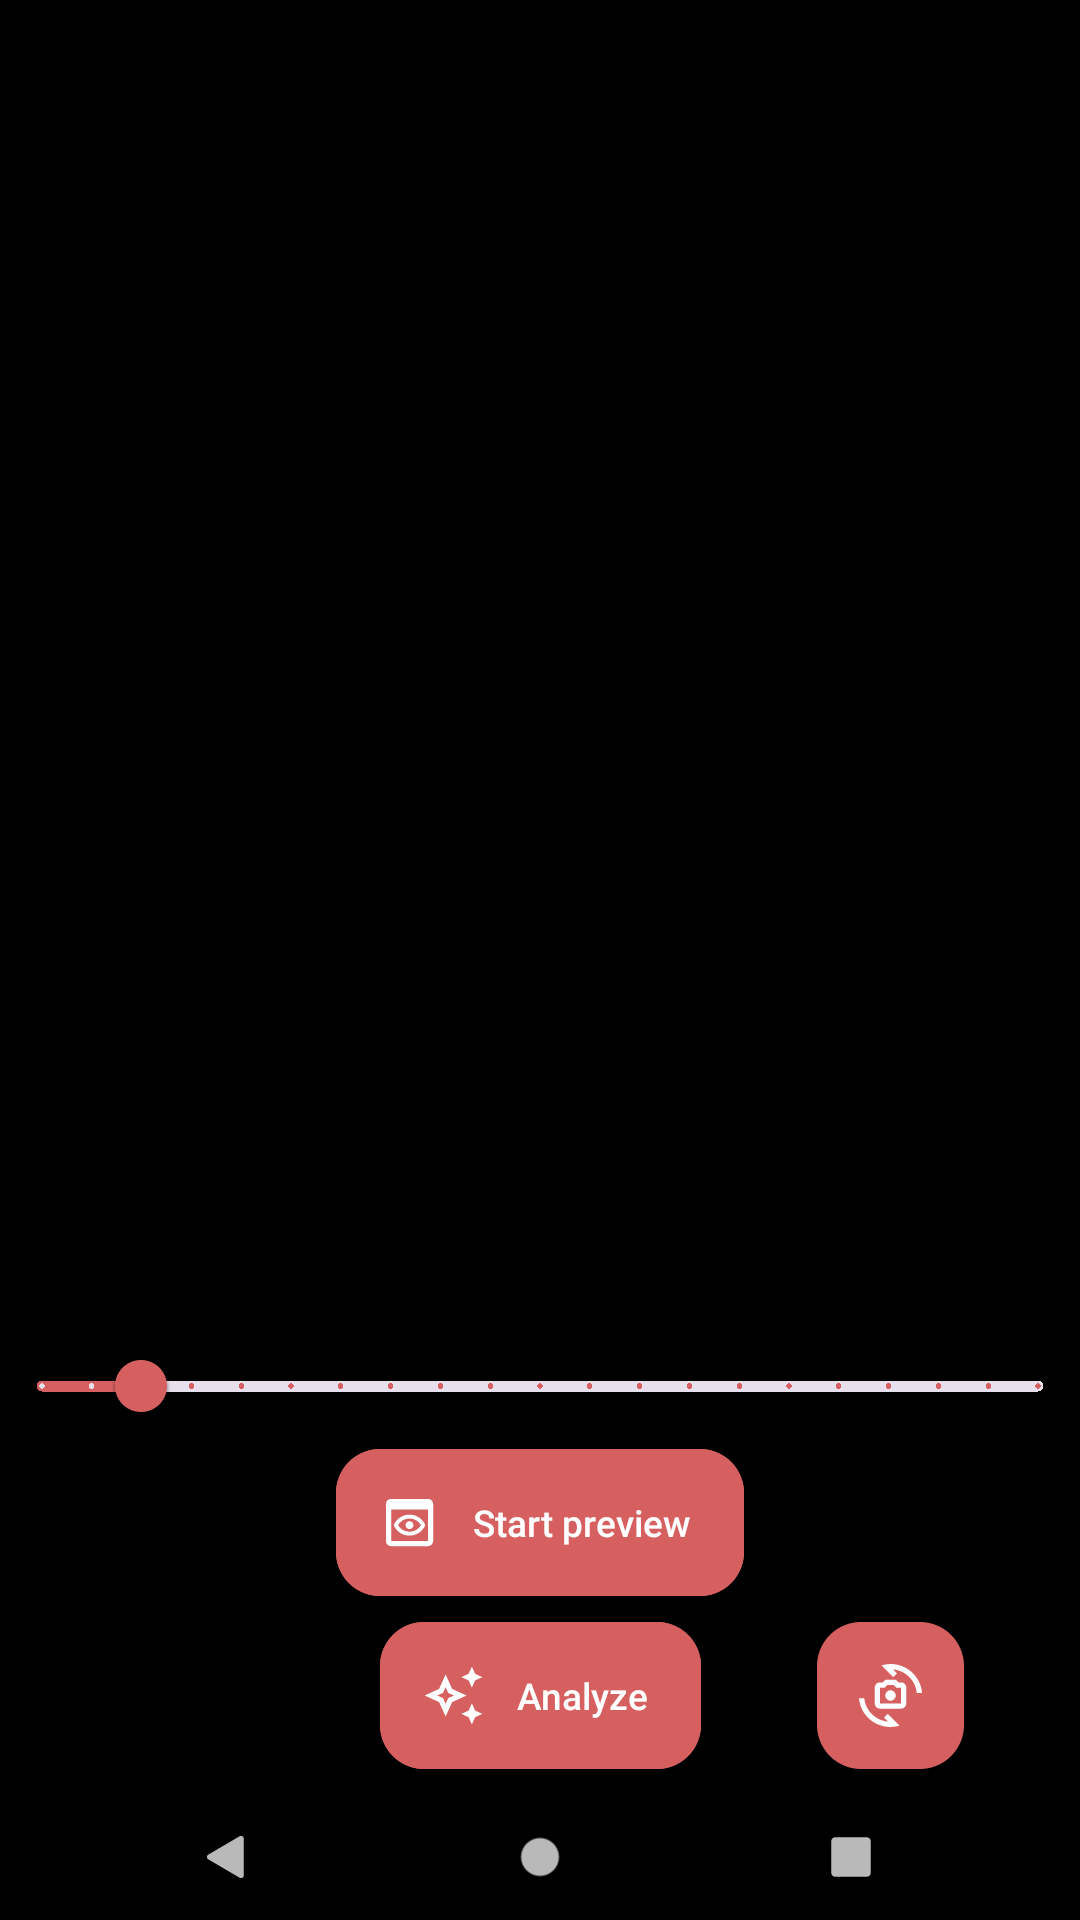
\includegraphics[scale=0.17]{img/nerd.png}
\end{figure}

\newpage
\subsubsection{Bottone Analyze}
Bottone premuto una volta avviata la \textit{Preview}, ci permette di vedere per la prima volta la nostra rete addestrata al lavoro su Android.
È stata inserita anche una barra di scorrimento in modo tale da impostare e mostrare real time a schermo gli occhi individuati solo sopra una certo livello di precisione della rete. (0\% minimo - 100\% massimo). Su Android se si inquadrano bene gli occhi, in media si ha una precisione del 80\%. 
\newline
Chiaramente più viene allontanato il telefono dalla faccia, più cala la precisione, ma comunque la rete individua sempre e comunque gli occhi a meno che non si provino a nascondere gli occhi o ci si metta di profilo.

\begin{figure}[h]
\caption{Nerd mode con analyze attiva }
\centering
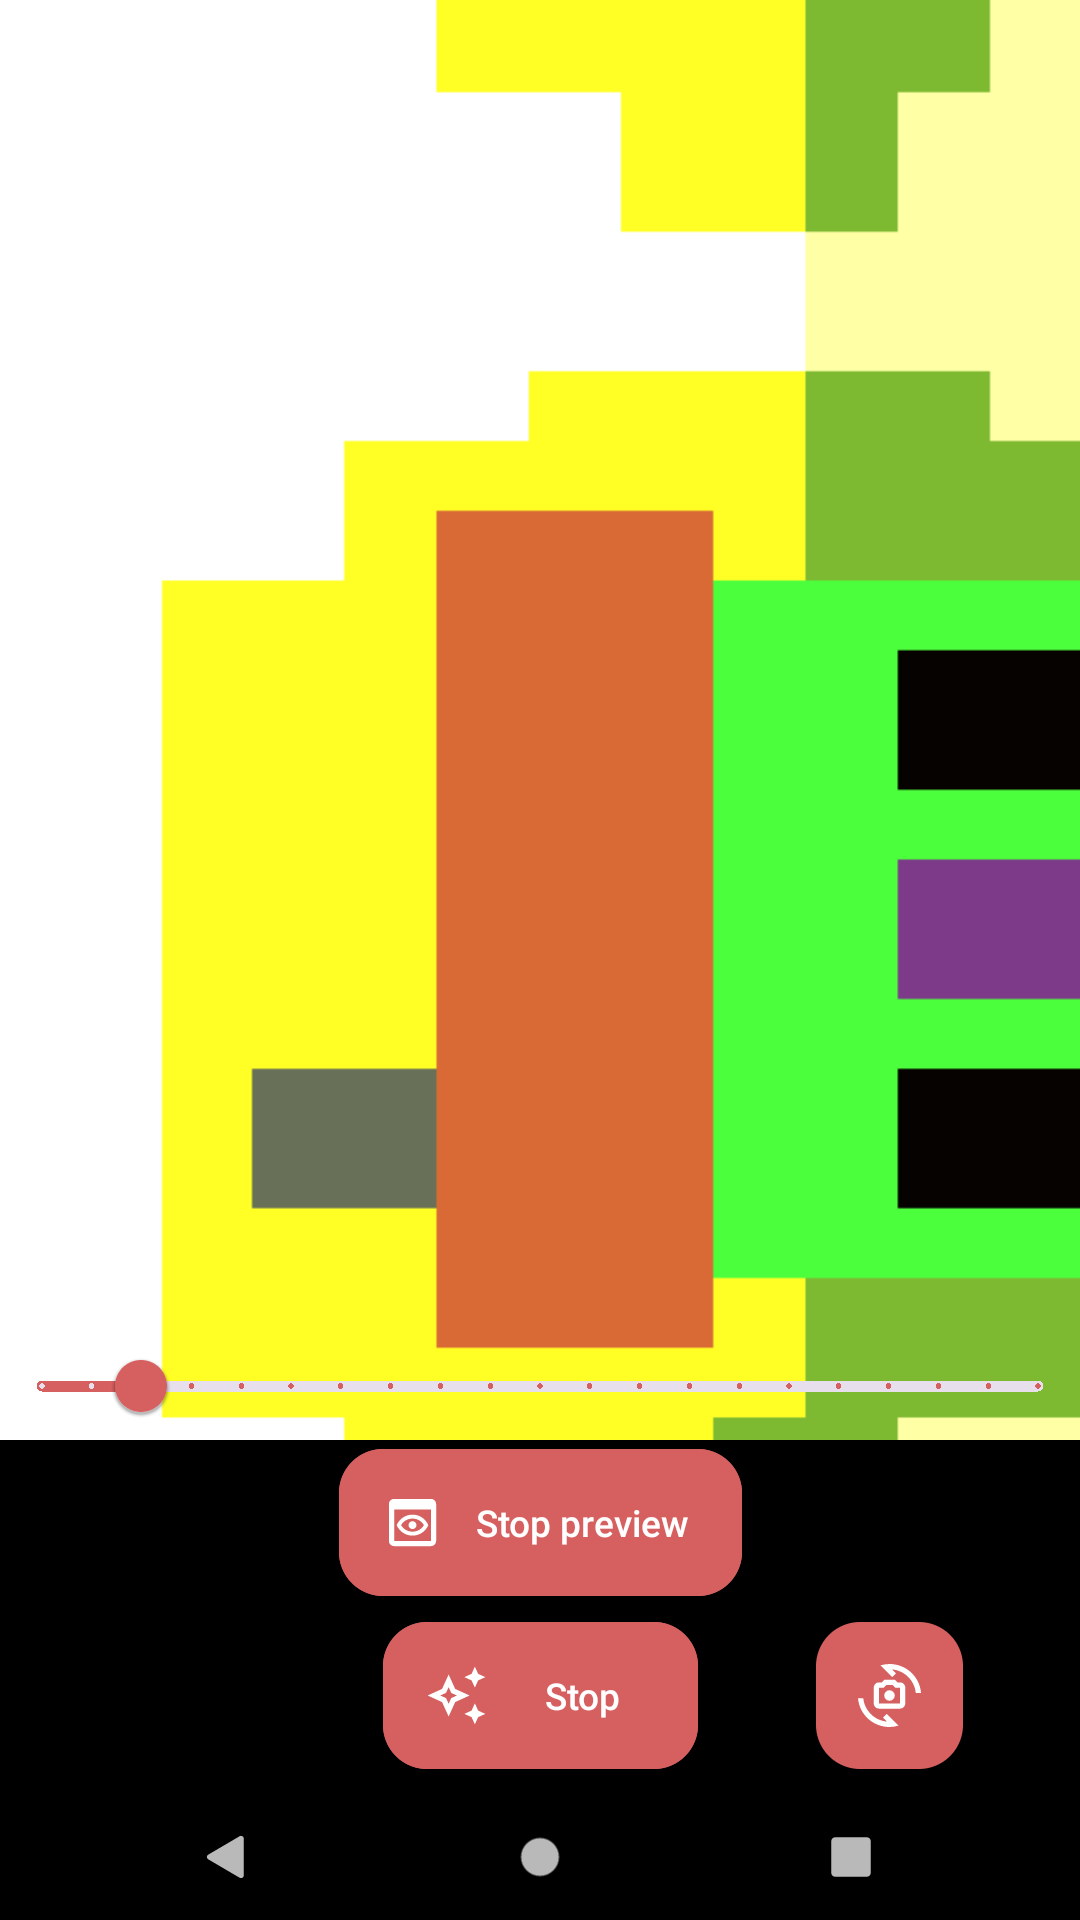
\includegraphics[scale=0.17]{img/analyze.png}
\end{figure}

\subsection{Calibration}
Modalità usata per calibrare al meglio la fotocamera e ottenere risultati i più veritieri possibili. Utile per svolgere al meglio il mini gioco descritto in seguito. Qui di sotto la sua schermata.


\begin{figure}[h]
\caption{Schermata Calibration }
\centering
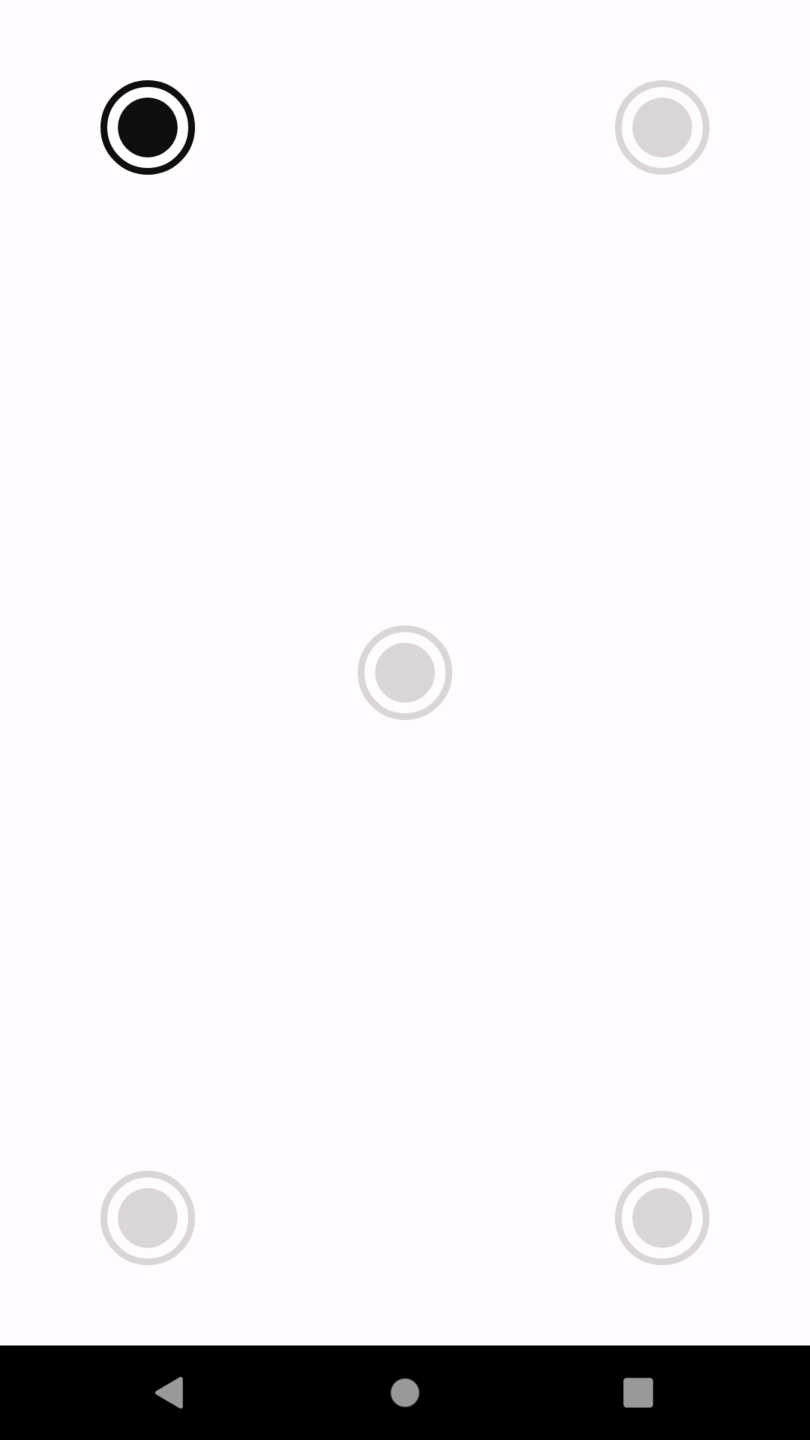
\includegraphics[scale=0.2]{img/calibration.png}
\end{figure}


\newpage
\subsection{Game}
Modalità usata per completare un mini-gioco sfruttando le potenzialità della rete neurale sottostante. Tramite un mini gioco Quiz infatti, l'utente può rispondere alle domande del Quiz semplicemente spostando il cellulare verso uno dei 4 angoli dove è posizionata la risposta corretta: infatti viene riconosciuto l'occhio e viene visualizzato un puntatore che lo identifica sullo schermo. La domanda viene posta al centro dello schermo per motivi pratici.
\newline
I dati delle domande e delle risposte sono state recuperate da uno dei tanti servizi di Api pubblici che si trovano in rete: tramite appunto una richiesta Url, vengono ricevuti i dati casuali in formato JSON per una singola domanda, e una volta ricevuta la risposta, corretta o sbagliata che sia, viene generata un'altra richiesta in modo tale da poter continuare il mini gioco. 
\begin{figure}[h]
	\centering
	\caption{Schermata Game}
	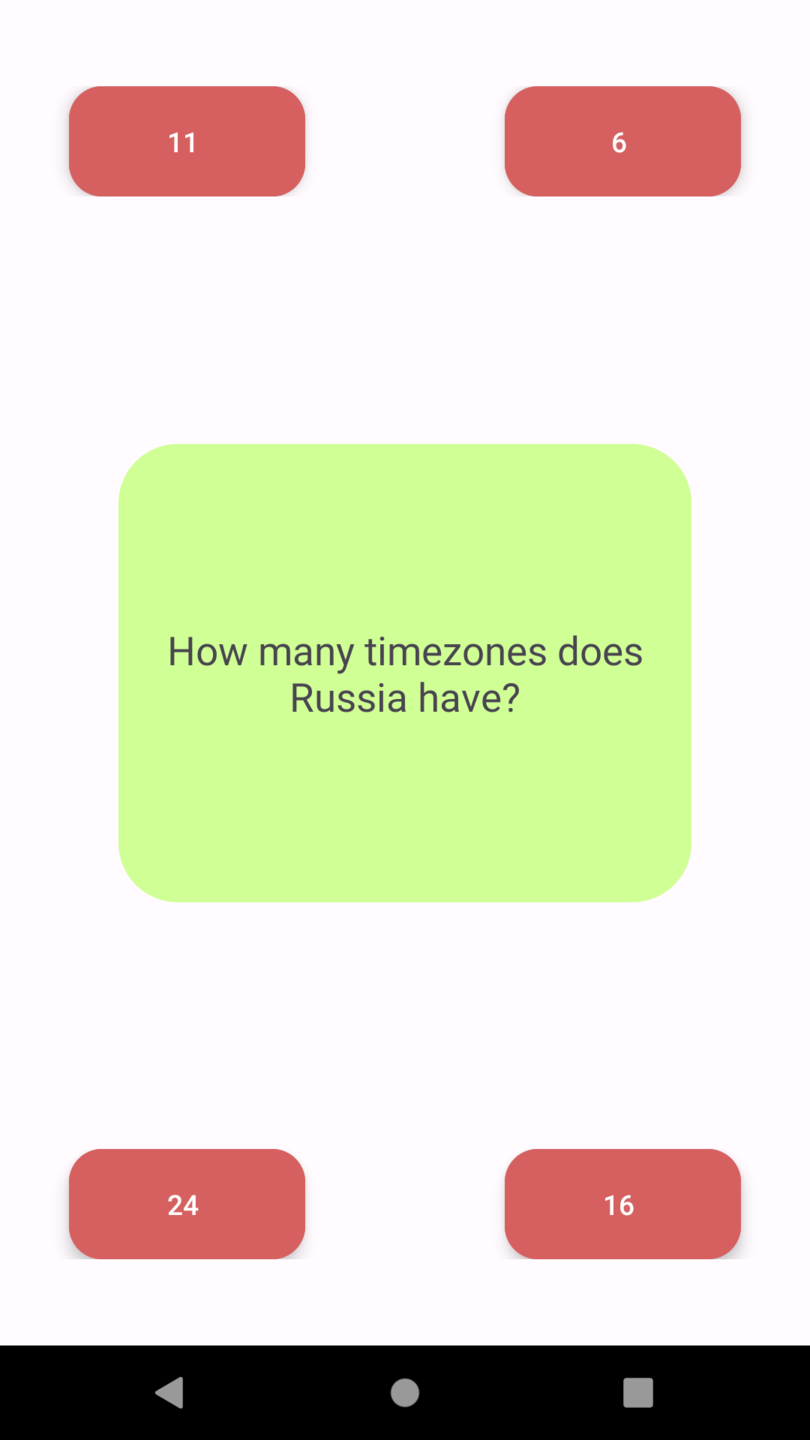
\includegraphics[scale=0.2]{img/game.png}
\end{figure}







\newpage
\section{Conclusioni}
Gli obiettivi del progetto sono stati raggiunti a pieno e con risultati soddisfacenti. 
\newline \newline
L’applicativo è
conforme alle aspettative e svolge i compiti adeguatamente.
Le parti realizzate
in Android risultano con prestazione adeguate.
\newline \newline
Il modello addestrato restituisce un output corretto la maggior parte delle volte con una precisione di eye tracking del 95\%.





\end{document}
